\pagebreak

Block name: SubbandArray

Number of inputs: 2

Number of outputs: 2

Parameter list: num\_of\_blk,SubbandArray\_Maxpfet,\\SubbandArray\_FBbias,SubbandArray\_FBpbias,SubbandArray\_FBnbias,\\SubbandArray\_FFbias,SubbandArray\_FFpbias,SubbandArray\_FFnbias,\\SubbandArray\_Maxota,SubbandArray\_LPF,SubbandArray\_FFcap,\\SubbandArray\_FBcap

Block description: 
Analog Front-end used to extract frequency spectrum of a signal. The block consists of band-pass filter, maximum detector and Low-pass filter. 
Inputs are all connected to one node. Outputs are vectorized to have M. 

\begin{figure}[H]  % jpg, png, or pdf
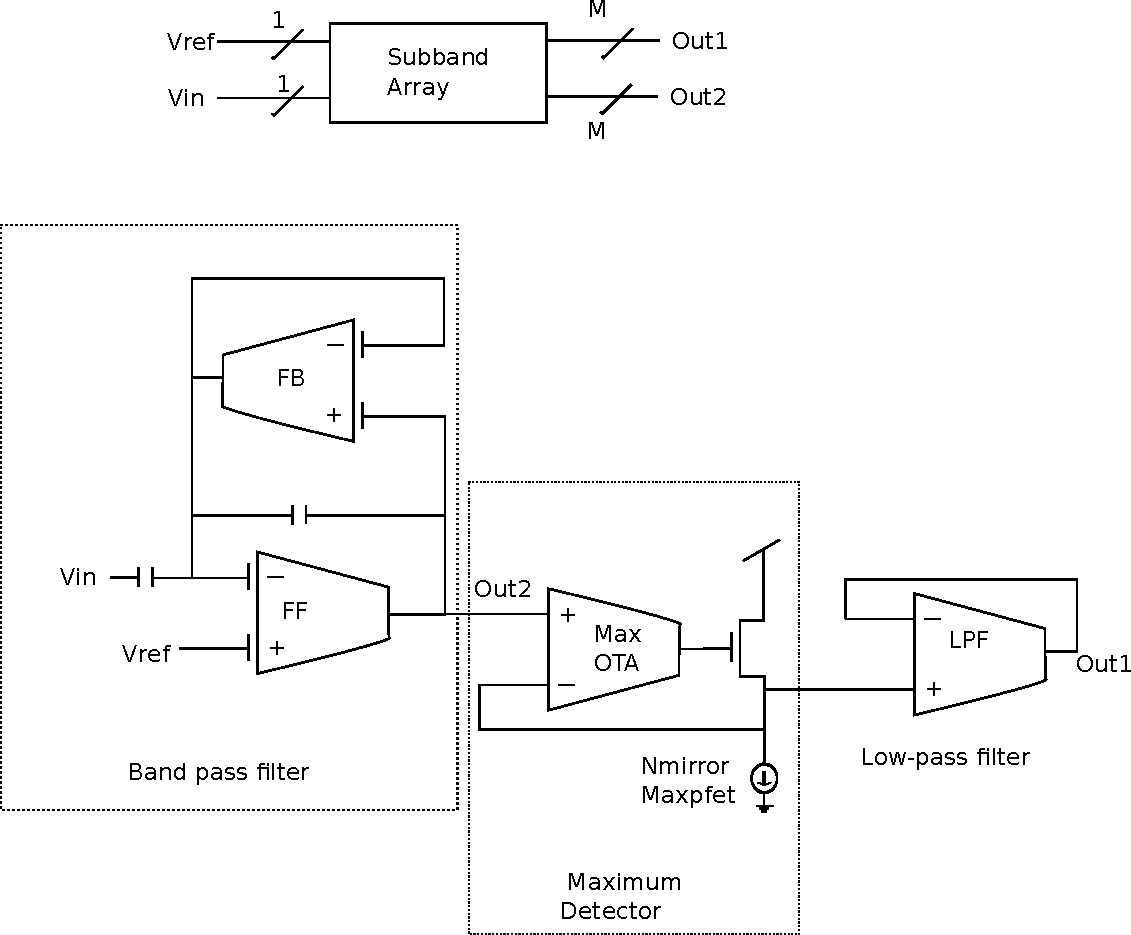
\includegraphics[width=300pt]{/home/ubuntu/rasp30/sci2blif/documentation/blocks_latex/figures/SubbandArray.pdf}
\end{figure}

